\documentclass[11pt]{article}
\usepackage[letterpaper,margin=1in]{geometry}
\usepackage[T1]{fontenc}
\usepackage{lmodern}
\usepackage[protrusion=true,expansion=true,stretch=25,shrink=25,step=5]{microtype}
\usepackage{titlesec}
\usepackage{amsmath}
\usepackage{booktabs,tabularx,longtable,array}
\usepackage{enumitem}
\usepackage[font=small,labelfont=bf]{caption}
\usepackage{xcolor}
\usepackage{listings}
\usepackage{graphicx}
\usepackage{placeins}
\usepackage{tikz}
\usetikzlibrary{arrows.meta,positioning,fit,calc,shapes.geometric,backgrounds,matrix}
\usepackage{pgfplots}
\pgfplotsset{compat=1.17}
\usepackage[hidelinks]{hyperref}

\widowpenalty=10000
\clubpenalty=10000
% last line of every paragraph at least 70% of the line width
\setlength{\parfillskip}{0pt plus 0.3\linewidth}
\setlength{\emergencystretch}{1.5em}
% headings and table cells use the normal fill
\newcommand{\normalfill}{\setlength{\parfillskip}{0pt plus 1fil}}
\titleformat*{\section}{\normalfont\Large\bfseries\normalfill}
\titleformat*{\subsection}{\normalfont\large\bfseries\normalfill}
\titleformat*{\subsubsection}{\normalfont\normalsize\bfseries\normalfill}
\captionsetup{justification=justified,singlelinecheck=true}
\DeclareCaptionFormat{pfill}{#1#2\setlength{\parfillskip}{0pt plus 0.3\linewidth}#3\par}
\captionsetup{format=pfill}
\setlength{\parskip}{4pt}
\setlist{itemsep=1pt,topsep=3pt}
\renewcommand{\arraystretch}{1.15}

\newcommand{\fw}[1]{\texttt{\detokenize{#1}}}
\newcommand{\sig}[1]{\texttt{\detokenize{#1}}}
\newcolumntype{L}{>{\raggedright\arraybackslash\normalfill}X}
\newcolumntype{P}[1]{>{\raggedright\arraybackslash\normalfill}p{#1}}

\definecolor{eng}{RGB}{220,232,245}
\definecolor{mem}{RGB}{235,225,245}
\definecolor{hst}{RGB}{226,240,226}
\definecolor{pinc}{RGB}{250,236,214}
\definecolor{okc}{RGB}{60,140,60}
\definecolor{badc}{RGB}{190,50,40}

\lstset{basicstyle=\ttfamily\small,columns=fullflexible,keepspaces=true,
  frame=single,framerule=0.3pt,xleftmargin=4pt,xrightmargin=4pt,
  commentstyle=\color{gray},morecomment=[l]{;}}

\tikzset{
  blk/.style={draw,rounded corners=2pt,align=center,minimum height=8mm,font=\small},
  arr/.style={-{Stealth[length=2mm]},thick},
  lbl/.style={font=\scriptsize,align=center}
}

\title{PE16: A Programmable Protocol Engine for IHP SG13CMOS5L\\[2pt]
\large Architecture, Firmware, and Verification Report}
\author{Jane Street Protocol Emulator ASIC Competition entry}
\date{Tiny Tapeout 8$\times$4 tiles \quad Submission deadline 18 January 2027}

% Figures refer to the screenshots retained in the main repository.
% Build from docs/report/ so paths resolve to fpga/results/screenshots/.
\newcommand{\pescreenshot}[3]{%
\begin{figure}[!htbp]
\centering
\includegraphics[width=0.96\linewidth,height=60mm,keepaspectratio]{../../fpga/results/screenshots/#1.png}%
\caption{#2}\label{#3}
\end{figure}}

\begin{document}
\maketitle

\begin{abstract}
PE16 is a four-engine programmable processor for cycle-accurate digital protocol signaling. Each 16-bit engine executes firmware with deadline-relative delays, configurable CRC computation, bit stuffing and destuffing, NRZI, and complementary differential output. Twenty-three firmware programs cover sixteen protocol families, including UART, SPI, I\textsuperscript{2}C, CAN, USB low speed, Modbus RTU, and MIL-STD-1553. Verilog, Python, and Lean~4 implementations of the instruction set are cross-checked through randomized execution, with eight Lean theorems establishing timing and stuffing properties. The expanded cocotb suite passes 36 top-level tests, including post-layout gate-level simulation. An IHP SG13CMOS5L 8$\times$4 Tiny Tapeout implementation with four SRAM macros completes GDS hardening, precheck, and LVS, with positive setup and hold slack at three corners under a 20\,ns clock constraint. A 48\,MHz Basys3 prototype further validates concurrent execution, host configuration, and physical protocol signaling.

%======================================================================
\end{abstract}

{\normalfill\tableofcontents}
\clearpage

%======================================================================
\section{Summary}

PE16 replaces multiple dedicated protocol controllers with four independent, firmware-programmed signaling engines. The hardware supplies the operations most protocols share---precise timing, bit shifting, programmable CRC, stuffing, and line coding---while firmware defines framing, transactions, and control flow. The host SPI interface loads and replaces programs, configures engines, and exchanges data without changing the hardware.

Table~\ref{tab:summary} summarizes the completed design and its verification.
\begin{table}[!htbp]
\centering\small
\caption{PE16 implementation summary.}\label{tab:summary}
\begin{tabularx}{\linewidth}{@{}lL@{}}
\toprule
Engines & Four independent 16-bit engines (two in the flip-flop fallback) \\
Instruction memory & Four IHP 256$\times$16 SRAM macros; independent per engine \\
Clock & 48\,MHz nominal; ASIC constrained to 20\,ns (50\,MHz) \\
Protocol I/O & Eight shared bidirectional pins with programmable ownership and validity \\
Host interface & SPI mode~0, up to one-eighth of the system clock \\
Firmware & 23 programs covering 16 protocol families \\
RTL and gate-level tests & 36 top-level cocotb tests passed \\
ISA models & Verilog, Python and Lean~4; 200 randomized RTL programs and 500 Lean traces \\
Formal properties & Eight Lean theorems, no \texttt{sorry} \\
Mutation tests & 19/20 RTL (one equivalent), 8/8 Lean, 28/37 firmware detected \\
ASIC area & 0.2212\,mm$^2$ standard cells + 0.1125\,mm$^2$ SRAM \\
Post-route timing & Worst setup $+6.344$\,ns; worst hold $+0.102$\,ns \\
Physical verification & Routed DRC 0, LVS 0, all Tiny Tapeout prechecks passed \\
FPGA & Four engines on Basys3 at 48\,MHz; eight saved WaveForms captures \\
\bottomrule
\end{tabularx}
\end{table}

The ISA and host command definitions are documented in \texttt{docs/isa.md}; the full protocol inventory is in \texttt{docs/protocols.md}, with detailed measured results in \texttt{docs/verification.md}.

%======================================================================
\section{Challenge constraints}

\paragraph{Process and area.}
PE16 targets IHP SG13CMOS5L~\cite{ihp} through Tiny Tapeout~\cite{tt} for the Jane Street protocol emulator ASIC competition~\cite{js}. The final allocation is 8$\times$4 tiles with a die outline of $1724.16\times710.64\,\mu$m (1.2253\,mm$^2$). Four compiled SRAM macros provide independent program storage without the area overhead of full flip-flop memories.

\paragraph{Pins.}
The Tiny Tapeout template provides eight dedicated inputs, eight dedicated outputs, and eight bidirectional pins. The SPI host occupies three input bits and one output bit; protocol signals use the eight bidirectional pins. Output ownership is assigned per pin, while all engines may sample the same physical inputs.

\begin{table}[!htbp]
\centering\small
\caption{Tiny Tapeout ports and PE16 assignments.}\label{tab:ports}
\begin{tabularx}{\linewidth}{@{}llllL@{}}
\toprule
Port & Width & Direction & PE16 use & Notes \\
\midrule
\sig{ui_in} & 8 & input & bits 0--2: SCK, CS\_N, MOSI & bits 3--7 reserved \\
\sig{uo_out} & 8 & output & bit 0: MISO, bits 1--3: status & bits 4--7 reserved \\
\sig{uio} & 8 & bidirectional & protocol pins & per-pin output enable \\
\sig{clk}, \sig{rst_n}, \sig{ena} & 1 each & input & clock, reset, enable & \\
\bottomrule
\end{tabularx}
\end{table}

Open-drain interfaces such as I\textsuperscript{2}C and 1-Wire release the pin through its output enable; their HIGH state is supplied by an external pull-up. Protocols requiring external physical-layer transceivers use the same engine-side digital interface.

\paragraph{Clocking.}
The nominal 48\,MHz engine clock gives 32 cycles per USB low-speed bit and provides a convenient timing base for the firmware. The host SPI is synchronized to this clock and supports SCK at most \sig{clk/8}. The ASIC physical flow uses a slightly stricter 20\,ns clock period, while FPGA hardware was operated at 48\,MHz.

%======================================================================
\section{System architecture}

Figure~\ref{fig:system} shows the top level.
A host microcontroller loads programs, sets configuration, and moves data through the SPI host port.
Four engines share eight protocol pins through exclusive output ownership.
A per-pin ownership mux selects one engine's output and output-enable signals, while a validity mask can leave any pin unassigned.
Every engine reads every pin through a two-flop synchroniser that removes metastability from the asynchronous inputs.

\begin{figure}[t]
\centering
\resizebox{\linewidth}{!}{%
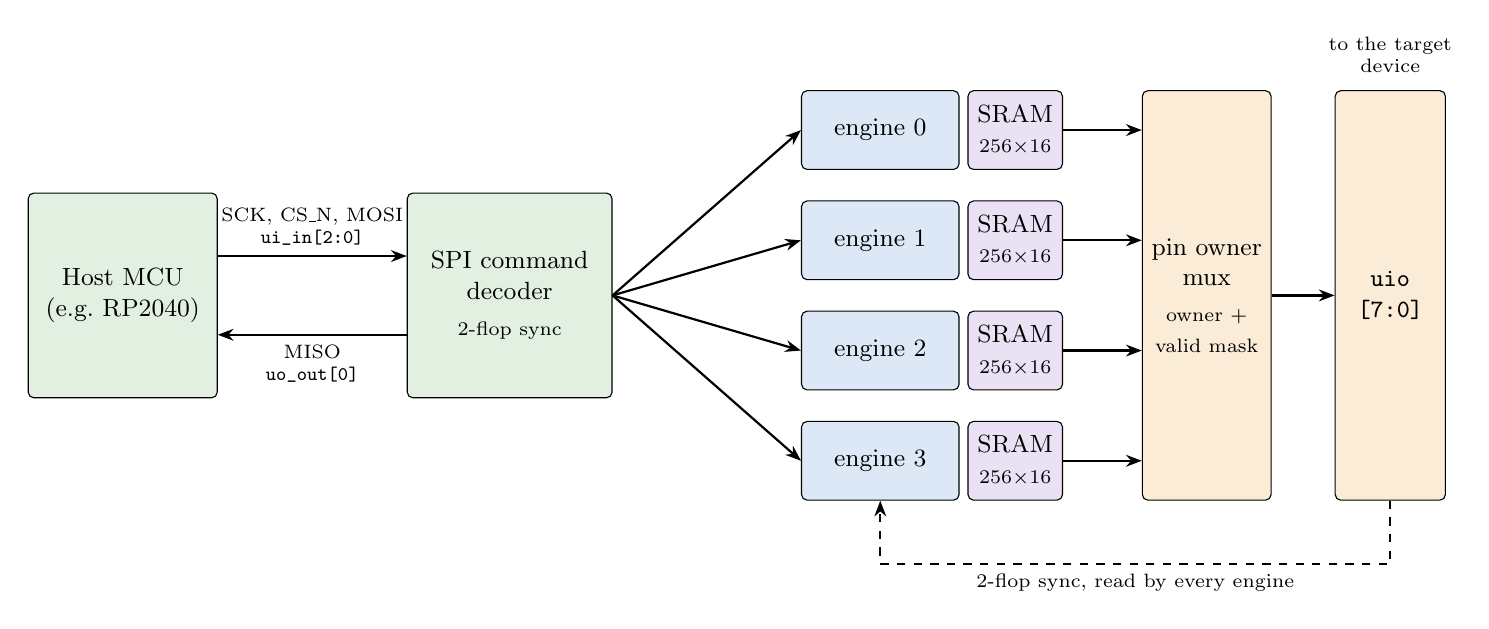
\begin{tikzpicture}[node distance=4mm]
  \node[blk,fill=hst,minimum width=24mm,minimum height=26mm] (host) {Host MCU\\(e.g.\ RP2040)};
  \node[blk,fill=hst,right=24mm of host,minimum width=26mm,minimum height=26mm] (spi) {SPI command\\decoder\\[2pt]\scriptsize 2-flop sync};
  \foreach \i/\y in {0/2.1,1/0.7,2/-0.7,3/-2.1}{
    \node[blk,fill=eng,minimum width=20mm,minimum height=10mm] (e\i) at ($(spi.east)+(3.4,\y)$) {engine \i};
    \node[blk,fill=mem,minimum width=12mm,minimum height=10mm,right=1mm of e\i] (m\i) {SRAM\\\scriptsize$256{\times}16$};
    \draw[arr] (spi.east) -- (e\i.west);
  }
  \node[blk,fill=pinc,minimum width=16mm,minimum height=52mm,right=10mm of m1.east|-spi] (or) {pin owner\\mux\\[2pt]\scriptsize owner +\\\scriptsize valid mask};
  \foreach \i in {0,1,2,3}{\draw[arr] (m\i.east) -- (or.west|-m\i);}
  \node[blk,fill=pinc,right=8mm of or,minimum width=14mm,minimum height=52mm] (pins) {\sig{uio}\\\sig{[7:0]}};
  \draw[arr] (or) -- (pins);
  \draw[arr,dashed] (pins.south) -- ++(0,-8mm) -| node[lbl,pos=0.25,below]{2-flop sync, read by every engine} (e3.south);
  \draw[arr] ([yshift=5mm]host.east) -- node[lbl,above]{SCK, CS\_N, MOSI\\\sig{ui_in[2:0]}} ([yshift=5mm]spi.west);
  \draw[arr] ([yshift=-5mm]spi.west) -- node[lbl,below]{MISO\\\sig{uo_out[0]}} ([yshift=-5mm]host.east);
  \node[lbl,above=1mm of pins] {to the target\\device};
\end{tikzpicture}}
\caption{Top level of the 4-engine build. Each engine has its own program memory, TX FIFO, and RX FIFO.}
\label{fig:system}
\end{figure}

\paragraph{Data path.}
The chip has no parallel data bus, so protocol data moves through the host port.
On transmit, words go from the host into an engine TX FIFO, then \texttt{PULL} moves a word into the output shift register \sig{osr}, and \texttt{OUT} shifts bits onto a pin.
On receive, \texttt{IN} shifts pin samples into the input shift register \sig{isr}, then \texttt{PUSH} moves it into the RX FIFO, and the host reads it on MISO.
Each FIFO holds four 16-bit words.
The host port accepts SCK up to one eighth of the system clock, which is 6\,MHz at 48\,MHz.

An engine stalls on \texttt{PULL} when its TX FIFO is empty and on \texttt{PUSH} when its RX FIFO is full.
Receive-heavy protocols such as JTAG, CAN receive, USB receive, Modbus receive, and 1553 receive therefore need the host to read the RX FIFO during the transfer.
The tests do this.

%======================================================================
\section{Engine RTL}

The engine is \texttt{src/pe\_core.v}, 227 lines of Verilog-2005.
Figure~\ref{fig:engine} shows its structure.

\begin{figure}[t]
\centering
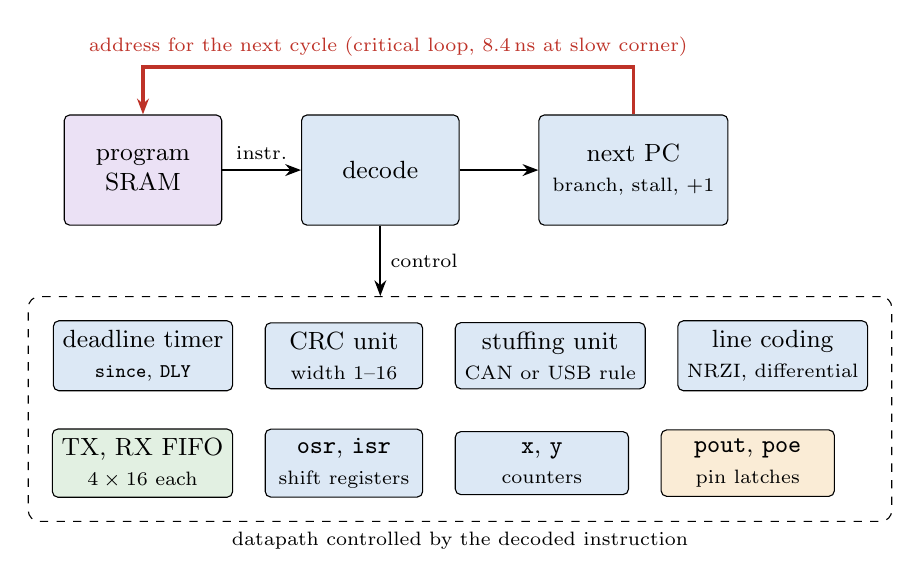
\begin{tikzpicture}[node distance=5mm]
  \node[blk,fill=mem,minimum width=20mm,minimum height=14mm] (ram) {program\\SRAM};
  \node[blk,fill=eng,right=10mm of ram,minimum width=20mm,minimum height=14mm] (dec) {decode};
  \node[blk,fill=eng,right=10mm of dec,minimum width=24mm,minimum height=14mm] (nxt) {next PC\\\scriptsize branch, stall, $+1$};
  \draw[arr] (ram) -- node[lbl,above]{instr.} (dec);
  \draw[arr] (dec) -- (nxt);
  \draw[arr,very thick,badc] (nxt.north) -- ++(0,6mm) -| node[lbl,pos=0.25,above,text=badc]{address for the next cycle (critical loop, 8.4\,ns at slow corner)} (ram.north);
  \node[blk,fill=eng,below=12mm of ram,minimum width=22mm] (dly) {deadline timer\\\scriptsize\sig{since}, \texttt{DLY}};
  \node[blk,fill=eng,right=4mm of dly,minimum width=20mm] (crc) {CRC unit\\\scriptsize width 1--16};
  \node[blk,fill=eng,right=4mm of crc,minimum width=22mm] (stf) {stuffing unit\\\scriptsize CAN or USB rule};
  \node[blk,fill=eng,right=4mm of stf,minimum width=22mm] (lc) {line coding\\\scriptsize NRZI, differential};
  \node[blk,fill=eng,below=5mm of crc,minimum width=20mm] (osr) {\sig{osr}, \sig{isr}\\\scriptsize shift registers};
  \node[blk,fill=eng,right=4mm of osr,minimum width=22mm] (xy) {\sig{x}, \sig{y}\\\scriptsize counters};
  \node[blk,fill=hst,left=4mm of osr,minimum width=22mm] (fifo) {TX, RX FIFO\\\scriptsize $4\times16$ each};
  \node[blk,fill=pinc,right=4mm of xy,minimum width=22mm] (pio) {\sig{pout}, \sig{poe}\\\scriptsize pin latches};
  \begin{scope}[on background layer]
    \node[draw,dashed,rounded corners,fit=(dly)(lc)(osr)(pio)(fifo),inner sep=3mm,label={[lbl]below:datapath controlled by the decoded instruction}] (dp) {};
  \end{scope}
  \draw[arr] (dec.south) -- node[lbl,right]{control} (dec.south|-dp.north);
\end{tikzpicture}
\caption{Engine structure. The program counter, decode, and next-PC logic form one combinational loop through the synchronous-read SRAM, and this loop sets the maximum clock frequency.}
\label{fig:engine}
\end{figure}

\subsection{Execution}
Every instruction retires in one cycle unless it stalls.
\texttt{WAIT} stalls until a pin has a given level, and \texttt{DLY} stalls until its deadline.
\texttt{PULL} stalls on an empty TX FIFO and \texttt{PUSH} on a full RX FIFO, while \texttt{HALT} stops the engine.
The program memory is a synchronous-read RAM.
The combinational next-PC value drives the RAM address, so the RAM output is the instruction for the next cycle.
This gives one instruction per cycle with no fetch bubble.

\subsection{Deadline timer}
The register \sig{since} counts cycles since the last \texttt{DLY} retired.
\texttt{DLY k} stalls until $\mathit{since}+1\ge k$ and then clears \sig{since}.
If $\mathit{since}+1>k$ on arrival, the deadline has passed and the sticky flag \sig{ov} is set.
Consecutive \texttt{DLY k} instructions therefore retire $k$ cycles apart, whatever path the code between them took, as long as that code takes fewer than $k$ cycles.
Firmware places each timed pin change on the cycle after a \texttt{DLY}, so edges fall on a fixed grid.
Figure~\ref{fig:dly} shows a loop body of four instructions under a deadline of 8 cycles.
\texttt{SET CTL sync} restarts the timer at an external event, for example right after a \texttt{WAIT} for a start bit.

\begin{figure}[t]
\centering
\resizebox{\linewidth}{!}{%
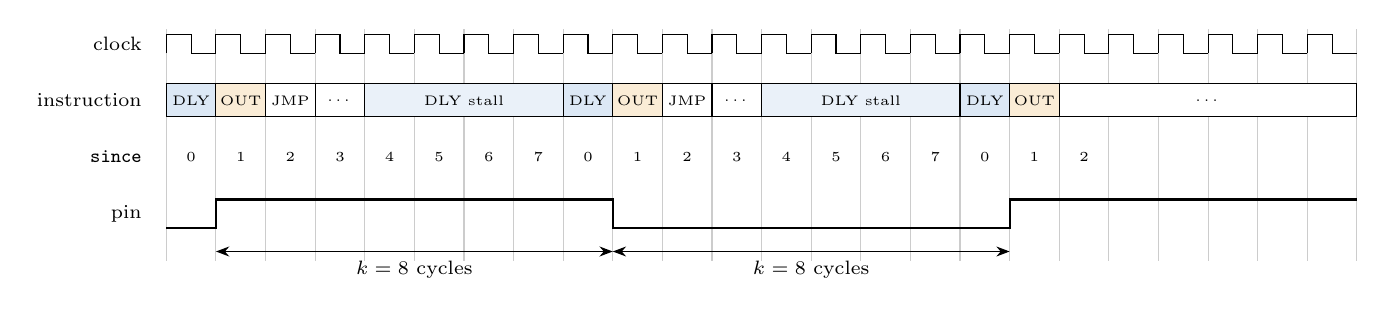
\begin{tikzpicture}[x=6.3mm,y=6mm]
  \foreach \t in {0,...,24}{\draw[gray!40] (\t,0.3) -- (\t,-4.6);}
  \node[lbl,anchor=east] at (-0.3,0) {clock};
  \foreach \t in {0,...,23}{\draw (\t,-0.2) -- (\t,0.2) -- (\t+0.5,0.2) -- (\t+0.5,-0.2) -- (\t+1,-0.2);}
  \node[lbl,anchor=east] at (-0.3,-1.2) {instruction};
  \foreach \s/\e/\n/\c in {0/1/DLY/eng,1/2/OUT/pinc,2/3/JMP/white,3/4/\ldots/white,4/8/DLY stall/eng!60,8/9/DLY/eng,9/10/OUT/pinc,10/11/JMP/white,11/12/\ldots/white,12/16/DLY stall/eng!60,16/17/DLY/eng,17/18/OUT/pinc,18/24/\ldots/white}{
    \draw[fill=\c] (\s,-1.55) rectangle (\e,-0.85); \node[font=\tiny] at ({(\s+\e)/2},-1.2) {\n};}
  \node[lbl,anchor=east] at (-0.3,-2.4) {\sig{since}};
  \foreach \t/\v in {0/0,1/1,2/2,3/3,4/4,5/5,6/6,7/7,8/0,9/1,10/2,11/3,12/4,13/5,14/6,15/7,16/0,17/1,18/2}{\node[font=\tiny] at (\t+0.5,-2.4) {\v};}
  \node[lbl,anchor=east] at (-0.3,-3.6) {pin};
  \draw[thick] (0,-3.9) -- (1,-3.9) -- (1,-3.3) -- (9,-3.3) -- (9,-3.9) -- (17,-3.9) -- (17,-3.3) -- (24,-3.3);
  \draw[{Stealth}-{Stealth}] (1,-4.4) -- node[lbl,below]{$k=8$ cycles} (9,-4.4);
  \draw[{Stealth}-{Stealth}] (9,-4.4) -- node[lbl,below]{$k=8$ cycles} (17,-4.4);
\end{tikzpicture}}
\caption{Deadline timing with \texttt{DLY 8}. The code after each retire takes a variable number of cycles, and the stall absorbs the difference. Pin edges follow each \texttt{DLY} by one cycle and are 8 cycles apart.}
\label{fig:dly}
\end{figure}

\subsection{CRC, stuffing, and line coding}
The CRC unit performs one serial step per \texttt{OUT crc}, \texttt{OUT stuff}, \texttt{IN crc}, or \texttt{IN destuff}, with width 1 to 16 and the polynomial set by the host.
Width 1 with polynomial 1 gives a parity bit.
Reflected CRCs such as USB and Modbus are fed in line order and then bit-reversed with \texttt{MOV @}.
\texttt{MOV \^{}} left-justifies a CRC of any width and fills the freed low bits with ones, and \texttt{JMP cz} tests for a zero remainder at the end of a received frame.

The stuffing unit counts either equal consecutive bits (CAN) or ones (USB and HDLC) up to \sig{stuff_n}.
\texttt{OUT stuff} places either a stuff bit or the next data bit.
A stuff bit consumes no \sig{osr} bit, skips the CRC, and sets flag \sig{s}.
\texttt{IN destuff} discards a stuff bit and sets \sig{s}.
Firmware repeats the bit slot with \texttt{JMP s}, and \texttt{JMP due} tests whether a stuff bit is pending at the end of a field.
With \sig{nrzi} set, \texttt{OUT} drives NRZI and \texttt{IN} decodes against the last sampled level.
With \sig{diff} set, \texttt{OUT} also drives pin $i{+}1$ with the complement.
\texttt{IN peek} always returns the raw pin level, which USB needs to detect SE0.

%======================================================================
\section{Top level and program memory}

\subsection{Host command set}
The host uses SPI mode~0 with an eight-bit command byte \sig{{engine[1:0],code[5:0]}}, transmitted MSB-first. Bits~7--6 address the engine and bits~5--0 select an operation. Word payloads and readbacks are 16 bits, MSB-first. The port supports live FIFO service while an engine runs; instruction-memory writes are accepted only when the selected engine is stopped.

\begin{table}[!htbp]
\centering\small
\caption{SPI host commands.}\label{tab:cmds}
\begin{tabularx}{\linewidth}{@{}clL@{}}
\toprule
Code & Command & Payload or response \\
\midrule
1 & program write & address byte, then 16-bit instructions with auto-increment \\
2 & configuration write & register byte, then 16-bit value \\
3 & TX push & one or more 16-bit words \\
4 & RX pop & reads 16-bit words (zero if empty) \\
5 & status & current PC, RUN, HALT and timing overrun \\
6 & FIFO counts & RX count in bits 5--3; TX count in bits 2--0 \\
7 & control & one byte: bit 0 RUN, bit 1 engine reset \\
8 & owner read & reads the global 16-bit pin-owner register \\
9 & configuration read & register byte, then 16-bit readback \\
\bottomrule
\end{tabularx}
\end{table}

\subsection{Configuration and pin ownership}
Per-engine configuration register~0 stores the CRC polynomial. Register~1 selects CRC width, shift directions, stuffing threshold and mode, NRZI, and complementary output. The CRC-width field encodes the width minus one. Register~1 resets to \texttt{0x03F}, selecting a 16-bit CRC, LSB-first shifts, and disabled stuffing and line coding.

Global register~2, written through Engine~0, holds \sig{PIN_OWNER}. For each physical pin $p$, bits $[2p+1:2p]$ identify its driving engine. Global register~3, \sig{PIN_VALID}, enables each assignment independently. With \sig{PIN_VALID[p]} cleared, physical output enable is zero regardless of engine state. When valid, the selected engine's \sig{pout[p]} and \sig{poe[p]} control the output. Every engine receives the synchronized physical input, independent of its output ownership.

For example, writing \texttt{02 02 00 E4} assigns pins~0--3 to Engines~0--3 respectively, and \texttt{02 03 00 0F} enables those four assignments. Command~9 reads either register back; command~8 provides direct owner readback. Global reset clears both routing registers, leaving all protocol outputs high-impedance. Engine-specific resets preserve the global routing configuration.

\subsection{Program memory builds}
The ASIC build uses four \sig{RM_IHPSG13_1P_256x16_c2_bm_bist} single-port SRAM macros through \texttt{src/pe\_imem.v}. Each macro is read synchronously at the address selected by the engine's next-PC logic and written from the host when the engine is stopped. The wrapper also supports a behavioral 256-word model and a two-engine, 128-word flip-flop fallback.

The final physical configuration explicitly places the four macros and connects their power pins through a customized LibreLane power-distribution step. Macro LEF, Liberty and GDS views, positions, and PDN connections are specified in \texttt{src/config.json}. The full GDS flow completed using the SRAM configuration, making the four-engine build the implemented ASIC design. The Basys3 prototype instead infers four block RAMs with matching synchronous fetch timing.

The original firmware programs contain at most 96 instructions, so each fits within both the SRAM and reduced-memory builds.

%======================================================================
\section{Instruction set and assembler}

Instructions are 16 bits with the opcode in bits [15:13], as listed in Table~\ref{tab:isa}.
The full encoding, with every field of every instruction, is in \texttt{docs/isa.md}.

\begin{table}[h]
\centering\small
\caption{Instruction set.}\label{tab:isa}
\begin{tabularx}{\linewidth}{@{}clL@{}}
\toprule
Op & Mnemonic & Function \\
\midrule
0 & \texttt{JMP} & conditions always, \texttt{x0}, \texttt{x-{}-}, \texttt{y0}, \texttt{y-{}-}, \texttt{b}, \texttt{s}, \texttt{cz}, \texttt{x!=y}, \texttt{due}, \texttt{txe} \\
1 & \texttt{WAIT} & stall until a pin has a given level \\
2 & \texttt{DLY} & deadline delay, immediate up to 4095 or the value in \texttt{x} \\
3 & \texttt{OUT} & raw, crc, stuff, or oe: one \sig{osr} bit to a pin or its output enable \\
4 & \texttt{IN} & raw, crc, destuff, or peek: one pin sample into \sig{isr} or flag \sig{b} \\
5 & \texttt{SET} & a pin, an enable, all pins, all enables, \texttt{x}, \texttt{y}, or control flags \\
6 & \texttt{MOV} & register move with optional invert, CRC alignment, and bit reversal \\
7 & \texttt{PULL}, \texttt{PUSH}, \texttt{HALT}, \texttt{NOP} & FIFO access and stop \\
\bottomrule
\end{tabularx}
\end{table}

The two-pass assembler in \texttt{isa/pe16.py} supports labels, \texttt{.equ} constants, and expressions evaluated at the design clock.
The helpers \texttt{ns}, \texttt{us}, and \texttt{ms} round up to whole cycles, and \texttt{bit(baud)} rounds to the nearest cycle.
Firmware timing is written as time, for example \texttt{dly \{us(70)\}}, so a change of \texttt{CLOCK\_HZ} retimes every program.
The assembler rejects \texttt{DLY} values outside 1 to 4095 and \texttt{SET} immediates outside 0 to 1023.
This range check caught two out-of-range constants during development.

%======================================================================
\section{Firmware techniques}

\paragraph{Deadline-timed edges.}
Each timed pin change sits on the cycle after a \texttt{DLY}.
Branches, word pulls, and counter updates in between add no timing error while they fit inside the delay.

\paragraph{Parity in the program counter.}
The ISA has no parity unit, while Modbus RTU and MIL-STD-1553 need parity next to a CRC or with none.
Each bit loop exists in two copies for an even and an odd count of ones so far, as in Figure~\ref{fig:parity}.
A 1 bit moves execution to the other copy, and the copy reached at the parity slot decides the parity bit.
The receivers check parity the same way.

\begin{figure}[h]
\centering
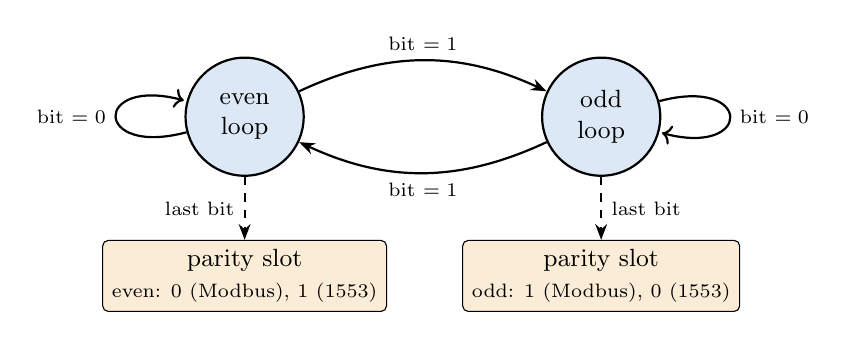
\begin{tikzpicture}[node distance=30mm,
  st/.style={circle,draw,thick,minimum size=15mm,align=center,font=\small,fill=eng}]
  \node[st] (E) {even\\loop};
  \node[st,right=of E] (O) {odd\\loop};
  \draw[arr] (E) edge[bend left=25] node[lbl,above]{bit $=1$} (O);
  \draw[arr] (O) edge[bend left=25] node[lbl,below]{bit $=1$} (E);
  \draw[arr] (E) edge[loop left] node[lbl,left]{bit $=0$} (E);
  \draw[arr] (O) edge[loop right] node[lbl,right]{bit $=0$} (O);
  \node[blk,below=8mm of E,fill=pinc] (pe) {parity slot\\\scriptsize even: 0 (Modbus), 1 (1553)};
  \node[blk,below=8mm of O,fill=pinc] (po) {parity slot\\\scriptsize odd: 1 (Modbus), 0 (1553)};
  \draw[arr,dashed] (E) -- node[lbl,left]{last bit} (pe);
  \draw[arr,dashed] (O) -- node[lbl,right]{last bit} (po);
\end{tikzpicture}
\caption{Parity tracked by program location. The CRC unit stays free for the frame CRC.}
\label{fig:parity}
\end{figure}

\paragraph{Open drain and the scratch pin.}
For open-drain lines the output value stays 0 and firmware toggles only the output enable.
Some programs test the next \sig{osr} bit by shifting it onto pin 7 with its output disabled, which sets flag \sig{b} without driving the pin.
The pin-ownership mux prevents these internal scratch writes from changing an output owned by another engine.

\paragraph{Edge-detection latency.}
A receiver that starts its bit timer on a detected edge starts it 3 cycles late, because of the two synchroniser flip-flops and the \texttt{WAIT} cycle.
The UART and USB receivers subtract this latency from their half-bit delay.
Section~\ref{sec:uarttol} shows how a bit-rate sweep found this defect.

%======================================================================
\section{Protocols}

Figure~\ref{fig:pinmap} shows the pins used by each program.
Output ownership isolates each engine's pin latches; the host assigns distinct outputs for concurrent protocols. Every engine may sample all eight inputs.
Table~\ref{tab:protocols} lists rate, host interface, test evidence, and limits for every program.
A reference model in this section means pin-level Python code in the testbench, written from the protocol specification, with no access to engine state.

\begin{figure}[h]
\centering
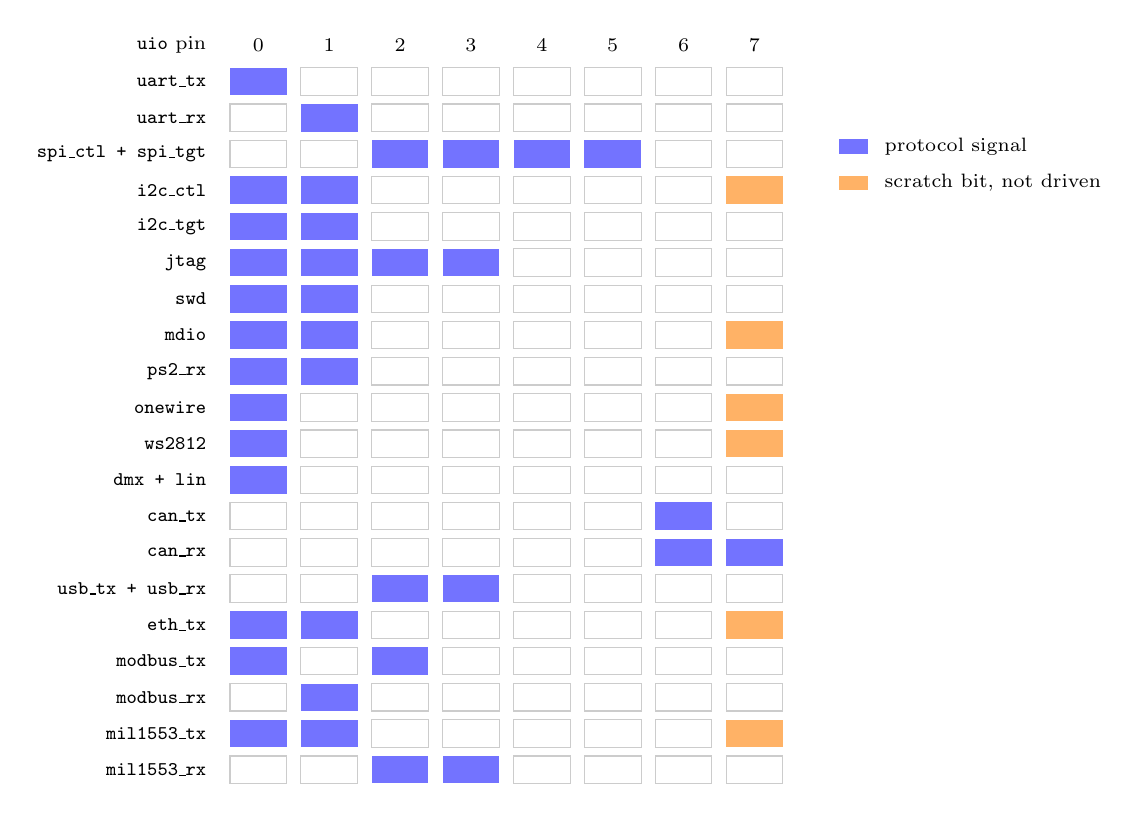
\begin{tikzpicture}[x=9mm,y=4.6mm]
  % pin usage: 1 = signal, 2 = scratch
  \def\use{{{1,0,0,0,0,0,0,0},{0,1,0,0,0,0,0,0},{0,0,1,1,1,1,0,0},{1,1,0,0,0,0,0,2},{1,1,0,0,0,0,0,0},{1,1,1,1,0,0,0,0},{1,1,0,0,0,0,0,0},{1,1,0,0,0,0,0,2},{1,1,0,0,0,0,0,0},{1,0,0,0,0,0,0,2},{1,0,0,0,0,0,0,2},{1,0,0,0,0,0,0,0},{0,0,0,0,0,0,1,0},{0,0,0,0,0,0,1,1},{0,0,1,1,0,0,0,0},{1,1,0,0,0,0,0,2},{1,0,1,0,0,0,0,0},{0,1,0,0,0,0,0,0},{1,1,0,0,0,0,0,2},{0,0,1,1,0,0,0,0}}}
  \foreach \p in {0,...,7}{\node[font=\scriptsize] at (\p,1) {\p};}
  \node[font=\scriptsize,anchor=east] at (-0.6,1) {\sig{uio} pin};
  \foreach \r/\name in {0/uart\_tx,1/uart\_rx,2/spi\_ctl + spi\_tgt,3/i2c\_ctl,4/i2c\_tgt,5/jtag,6/swd,7/mdio,8/ps2\_rx,9/onewire,10/ws2812,11/dmx + lin,12/can\_tx,13/can\_rx,14/usb\_tx + usb\_rx,15/eth\_tx,16/modbus\_tx,17/modbus\_rx,18/mil1553\_tx,19/mil1553\_rx}{
    \node[font=\scriptsize\ttfamily,anchor=east] at (-0.6,-\r) {\name};
    \foreach \p in {0,...,7}{
      \pgfmathtruncatemacro{\u}{\use[\r][\p]}
      \ifnum\u=1 \fill[blue!55] (\p-0.4,-\r-0.38) rectangle (\p+0.4,-\r+0.38);
      \else\ifnum\u=2 \fill[orange!60] (\p-0.4,-\r-0.38) rectangle (\p+0.4,-\r+0.38);
      \else \draw[gray!40] (\p-0.4,-\r-0.38) rectangle (\p+0.4,-\r+0.38);\fi\fi
    }
  }
  \fill[blue!55] (8.2,-2) rectangle (8.6,-1.6); \node[font=\scriptsize,anchor=west] at (8.7,-1.8) {protocol signal};
  \fill[orange!60] (8.2,-3) rectangle (8.6,-2.6); \node[font=\scriptsize,anchor=west] at (8.7,-2.8) {scratch bit, not driven};
\end{tikzpicture}
\caption{Pin use per program on \sig{uio[7:0]}. Pin numbers are fixed in each program and can be moved with a small firmware edit.}
\label{fig:pinmap}
\end{figure}

{\small
\begin{longtable}{@{}P{25mm}P{19mm}P{31mm}P{40mm}P{26mm}@{}}
\caption{Protocol programs at 48\,MHz.}\label{tab:protocols}\\
\toprule
Program & Rate & Host interface & Test evidence & Limits \\
\midrule\endfirsthead
\toprule
Program & Rate & Host interface & Test evidence & Limits \\
\midrule\endhead
\bottomrule\endfoot
\fw{uart_tx}~\cite{rs232} & 16 clocks per bit as shipped & one byte per word & 4 bytes decoded, every edge on the 16-clock grid & no parity option \\
\fw{uart_rx}~\cite{rs232} & 16 clocks per bit & byte in bits [15:8] & 7 bytes at $\pm5\%$ bit-rate error & no break detection \\
\fw{spi_ctl}~\cite{spi} & 3\,MHz SCK & byte in, byte out & 3 bytes each way, slow target model & mode 0 only \\
\fw{spi_tgt}~\cite{spi} & external SCK, tested 1.5\,MHz & reply byte in, byte out & 3 bytes each way & half period above about 5 clocks \\
\fw{i2c_ctl}~\cite{i2c} & 400\,kHz fast mode & \sig{{S,P,R,A,data}} per byte & write, read with ACK and NACK, absent device, clock stretch, SCL low $\ge1.5\,\mu$s & 7-bit addresses, no arbitration \\
\fw{i2c_tgt}~\cite{i2c} & external SCL, tested 600\,kHz & reply byte in, byte out & write, read, other address ignored & one byte per transfer \\
\fw{jtag}~\cite{jtag} & 3\,MHz TCK & TMS and TDI pairs in, TDO out & IDCODE read from a TAP model & host builds the TAP path \\
\fw{swd}~\cite{swd} & 3\,MHz & reset length, request & DPIDR read, ACK, parity & reads only \\
\fw{mdio}~\cite{mdio} & MDC 2.4\,MHz & header and data words & write, read-back, PHY ID, MDC period 417\,ns & Clause 22 only \\
\fw{ps2_rx}~\cite{ps2} & device clock, tested 20\,kHz & 11-bit frame out & 2 scan codes & receive only \\
\fw{onewire}~\cite{onewire} & standard speed & reset, write, or read op & reset, presence, Read ROM, all pulses in spec & no overdrive \\
\fw{ws2812}~\cite{ws2812} & 800\,kHz & GRB bit stream & high 417 or 813\,ns, period 1.25\,$\mu$s & host keeps FIFO fed \\
\fw{dmx}~\cite{dmx} & 250\,kbaud 8N2 & slot count, bytes & break 90\,$\mu$s, MAB 12\,$\mu$s, 5 slots & transmit only \\
\fw{lin}~\cite{lin} & 19.2\,kbaud & byte count, bytes & break 13 bits, PID and checksum checked & host computes PID \\
\fw{can_tx}~\cite{can} & 500\,kb/s & bit count, frame bits & 12 frames bit-exact vs.\ a builder from ISO 11898-1~\cite{can} & no arbitration monitor \\
\fw{can_rx}~\cite{can} & 500\,kb/s & header, DLC, bytes, status & 5 frames ACKed, corrupted frame rejected & $\pm0.7\%$ rate tolerance \\
\fw{usb_tx}~\cite{usb} & 1.5\,Mb/s & PID, bit count, data & 4 packets match reference line states & packets only \\
\fw{usb_rx}~\cite{usb} & 1.5\,Mb/s & residue constant in & DATA0 accepted, corrupted rejected, token & $+0.4/-0.6\%$ tolerance \\
\fw{eth_tx}~\cite{mdio} & 2\,Mb/s Manchester & bit count, whole frame & 208-bit frame, link pulse every 16.000\,ms & not 10\,Mb/s \\
\fw{modbus_tx}~\cite{modbus1} & 115200 8E1 & byte count, bytes & CRC \texttt{76 87} for the standard example frame, gap 1759\,$\mu$s & 8E1 only \\
\fw{modbus_rx}~\cite{modbus1} & 115200 8E1 & silence count in & status 0, 1, and 2 cases, recovery & no t1.5 check \\
\fw{mil1553_tx}~\cite{mil1553} & 1\,Mb/s & word count, words & 160 half-bits match, edges on 500\,ns grid & word level only \\
\fw{mil1553_rx}~\cite{mil1553} & 1\,Mb/s & data and status words & parity and Manchester errors on every decoder path & $-0.25/+0.7\%$ tolerance \\
\end{longtable}
}

\subsection{Notes on selected protocols}

\paragraph{CAN.}
The transmitter runs \texttt{OUT stuff} per bit and repeats the slot after a stuff bit.
It left-justifies the CRC with \texttt{MOV \^{}}, so the trailing stuff bit and the CRC delimiter come out of one loop.
The receiver synchronises on SOF, destuffs every bit, branches on IDE for extended frames, and drives a dominant ACK only when the CRC remainder is zero.
The CRC-15 reference returns the catalogue check value 0x059E~\cite{reveng}.
The receiver samples at the bit centre, and CAN practice places the sample point at 75 to 87.5\% of the bit. Section~\ref{sec:tol} gives the measured bit-rate tolerance.

\paragraph{USB low speed.}
The 1.5\,Mb/s rate needs 32 clocks per bit, which fixed the system clock at 48\,MHz.
The transmitter sends the inverted and reversed CRC with \texttt{MOV \textasciitilde crc\^{}@} and adds a final stuff bit through \texttt{JMP due}.
The receiver finds SE0 with raw \texttt{IN peek} on both lines.
The tests confirmed the residue constants 0x800D and 0x0C, and the reference CRCs return the catalogue check values 0xB4C8 and 0x19~\cite{reveng}.

\paragraph{Modbus RTU.}
The engine appends CRC-16/MODBUS and keeps the line silent for 3.5 characters after each frame.
For the read-holding-registers frame \texttt{11 03 00 6B 00 03} it produces \texttt{76 87}, which matches the example frame republished in Modbus documentation~\cite{modbus2}.
The receiver counts silence in 16-clock polls to find the end of a frame and returns status 0 for a good CRC, 1 for a bad CRC, and 2 for a parity or framing error.

\paragraph{MIL-STD-1553.}
The transmitter sends command or status syncs and data syncs with Manchester II coding at 24 clocks per half-bit~\cite{mil1553}.
The receiver samples each half-bit near its centre, less the detection latency, and checks the sync shape, the mid-bit transition of every bit, and odd parity.
It decodes back-to-back words and recovers after an error.

\paragraph{Ethernet.}
Real 10BASE-T~\cite{mdio} needs about 2.4 clocks per half-bit at 48\,MHz, and the firmware loop needs 9 cycles on its longest path.
The program therefore runs at 2\,Mb/s and demonstrates framing, Manchester coding, and link pulses at one fifth of the 10BASE-T rate.

%======================================================================
\section{Verification}

\subsection{Approach}
Figure~\ref{fig:verif} shows how the checks relate.
The RTL and the Python model run in lock step on random programs.
The Lean model replays random traces from the Python model, and the eight theorems hold for the Lean model.
The RTL connects to the Lean model through simulation only, so mutation testing measures how far the simulation reaches.
Protocol tests then check firmware and RTL at the pins through the real host port.

\begin{figure}[t]
\centering
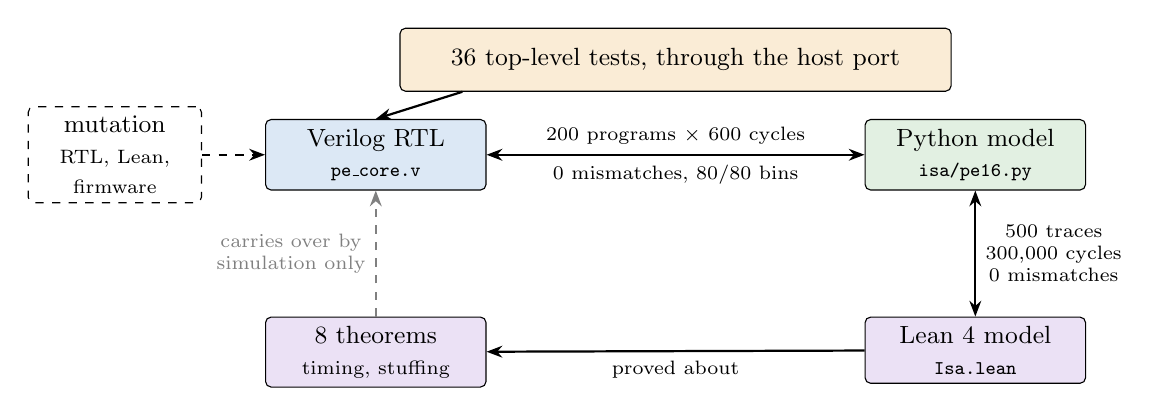
\begin{tikzpicture}[node distance=12mm]
  \node[blk,fill=eng,minimum width=28mm] (rtl) {Verilog RTL\\\scriptsize\texttt{pe\_core.v}};
  \node[blk,fill=hst,right=48mm of rtl,minimum width=28mm] (py) {Python model\\\scriptsize\texttt{isa/pe16.py}};
  \node[blk,fill=mem,below=16mm of py,minimum width=28mm] (lean) {Lean 4 model\\\scriptsize\texttt{Isa.lean}};
  \node[blk,fill=mem,below=16mm of rtl,minimum width=28mm] (thm) {8 theorems\\\scriptsize timing, stuffing};
  \draw[arr,{Stealth[length=2mm]}-{Stealth[length=2mm]}] (rtl) -- node[lbl,above]{200 programs $\times$ 600 cycles}node[lbl,below]{0 mismatches, 80/80 bins} (py);
  \draw[arr,{Stealth[length=2mm]}-{Stealth[length=2mm]}] (py) -- node[lbl,right]{500 traces\\300{,}000 cycles\\0 mismatches} (lean);
  \draw[arr] (lean) -- node[lbl,below]{proved about} (thm);
  \draw[arr,dashed,gray] (thm) -- node[lbl,left,text=gray]{carries over by\\simulation only} (rtl);
  \node[blk,fill=pinc,above=8mm of $(rtl)!0.5!(py)$,minimum width=70mm] (proto) {36 top-level tests, through the host port};
  \draw[arr] (proto.south west) ++(8mm,0) -- (rtl.north);
  \node[blk,fill=white,dashed,left=8mm of rtl,minimum width=22mm] (mut) {mutation\\\scriptsize RTL, Lean,\\\scriptsize firmware};
  \draw[arr,dashed] (mut) -- (rtl);
\end{tikzpicture}
\caption{Verification structure. Solid arrows are checks that run on every regression.}
\label{fig:verif}
\end{figure}

\subsection{RTL against the Python model}
The testbench in \texttt{test/core} runs 200 random programs of 600 cycles each.
The RTL engine and the Python model see the same random pins and host FIFO traffic, and all 18 state fields are compared every cycle.
The configuration is random across CRC width and polynomial, shift directions, stuffing mode and length, NRZI, and differential output.
Thirty percent of the programs stress the stuffing unit, and branch conditions are drawn uniformly over all 12 encodings.
The result is 0 mismatches over 120,000 program cycles with all 80 functional coverage bins hit.

\subsection{Lean 4 model and theorems}
The Lean model in \texttt{lean/Pe16/Isa.lean} implements the same cycle step as the Python model, field for field.
A compiled Lean executable replayed 500 random traces of 600 cycles with 0 mismatches.
\texttt{\#print axioms} shows only \texttt{propext}, \texttt{Quot.sound}, and \texttt{Classical.choice}.
Table~\ref{tab:thm} lists the theorems together with what each one means for firmware.

{\small
\begin{longtable}{@{}P{29mm}P{69mm}P{56mm}@{}}
\caption{Lean theorems about the Lean model.}\label{tab:thm}\\
\toprule
Theorem & Statement & Meaning for firmware \\
\midrule\endfirsthead
\toprule
Theorem & Statement & Meaning for firmware \\
\midrule\endhead
\bottomrule\endfoot
\fw{dly_retire} & At \texttt{DLY k} with $\mathit{since}=c<k$, the engine retires after $k-c$ cycles for any pin and FIFO inputs, with $\mathit{since}=0$ and \sig{ov} unchanged. & Input activity cannot shorten or lengthen a waiting \texttt{DLY}. \\
\fw{dly_period} & With $\mathit{since}=m<k$ on arrival, the retire comes $k$ cycles after the previous one. & Bit periods hold for any branch path in the loop body. \\
\fw{since_incr} & Every instruction except \texttt{DLY} and \texttt{SET CTL sync} adds one to \sig{since}. & The cost of code between deadlines equals its instruction count. \\
\fw{no_long_runs} & In identical-bit mode with $1\le \mathit{stuff\_n}\le7$, any sequence of \texttt{OUT stuff} with any data puts at most $\mathit{stuff\_n}$ equal bits in a row on the line. & The CAN stuffing rule holds for all data. \\
\fw{roundtrip} & The bits that \texttt{IN destuff} accepts from the transmitted line equal the data bits that \texttt{OUT stuff} consumed, in order, in both modes and for any $\mathit{stuff\_n}$. & Stuffing and destuffing are inverses. \\
\fw{stuff1_livelock} & In identical-bit mode, $\mathit{stuff\_n}=1$ stuffs forever. & A configuration to forbid. \\
\fw{stuff_progress} & For $\mathit{stuff\_n}\ge2$ a stuff bit is never followed by another. & Transmission always progresses. \\
\fw{ones_stuffbit} & In USB mode the stuff bit equals \sig{~last} when the mode stays fixed after reset. & Proves the surviving RTL mutant equivalent. \\
\end{longtable}
}

The proofs do not cover RTL equivalence, the CRC unit, the FIFOs, or any firmware program.
The CRC unit is instead checked against published check values in the protocol tests.

\subsection{Mutation testing}
A mutation test injects one deliberate fault and checks that verification catches it.
A survivor means either a gap in the checks or a fault with no visible effect, and each survivor needs an argument.
Table~\ref{tab:mut} gives the results for the RTL, the Lean model, the firmware, and the top level.

\begin{table}[h]
\centering\small
\caption{Mutation testing results.}\label{tab:mut}
\begin{tabularx}{\linewidth}{@{}lcL@{}}
\toprule
Level & Detected & Faults \\
\midrule
RTL & 19 / 20 & timer flag, CRC alignment, run-length saturation, stuff threshold, \texttt{DLY} compare, CRC feedback, branch conditions, FIFO full, NRZI, differential output, bit reversal, peek, overrun threshold, CRC masking and preset, shift input \\
Lean model & 8 / 8 & saturation, alignment, \texttt{WAIT}, \texttt{x!=y}, NRZI, differential output, \texttt{due}, reversal \\
Firmware & 28 / 37 & at least one fault in each of the 23 programs, including faults aimed at timing checks and at every parity and Manchester decoder path \\
Top level & 2 / 2 & engine select ignored, pin outputs from engine 0 only (injected by hand) \\
\bottomrule
\end{tabularx}
\end{table}

The one RTL survivor writes the USB stuff bit as \sig{~last} instead of 0, and \fw{ones_stuffbit} proves the two equal.
Before any RTL mutant runs, the script confirms full coverage on the unmodified design at the same seed budget.
Both mutation scripts apply faults to private copies of the sources.
Table~\ref{tab:gaps} lists the gaps that mutation testing exposed.

\begin{table}[h]
\centering\small
\caption{Gaps found by mutation testing, all closed.}\label{tab:gaps}
\begin{tabularx}{\linewidth}{@{}P{45mm}LL@{}}
\toprule
Survivor & Cause & Fix \\
\midrule
run-length saturation (Lean) & random traces rarely held 7 equal bits & stuffing-stress programs and a coverage bin \\
\texttt{x!=y} inverted (RTL) & the branch never ran at the mutation seed budget & uniform branch generation and a baseline coverage gate \\
1553 receiver Manchester check & error words reached one of four check paths & error words for all four paths \\
1553 and Modbus receiver parity & parity errors used even weights only & odd-weight error cases \\
UART receiver sampling at the bit edge & the test sent bits at the receiver rate & $\pm5\%$ bit-rate error, which also found a firmware defect \\
SPI controller sampling before SCK rise & the target model answered within one clock & slow target model with a 104\,ns output delay \\
\bottomrule
\end{tabularx}
\end{table}

\subsection{UART receiver tolerance}\label{sec:uarttol}
The survivor that sampled near the bit edge led to a bit-rate sweep, shown in Figure~\ref{fig:tol}.
The original receiver failed at a transmitter 4\% fast, because edge detection starts its timer 3 cycles late.
Subtracting this latency from the half-bit delay gives a symmetric $\pm5\%$ window.
The test now sends bytes at $\pm5\%$, which detects both the edge-sampling mutant and the uncompensated delay.

\begin{figure}[h]
\centering
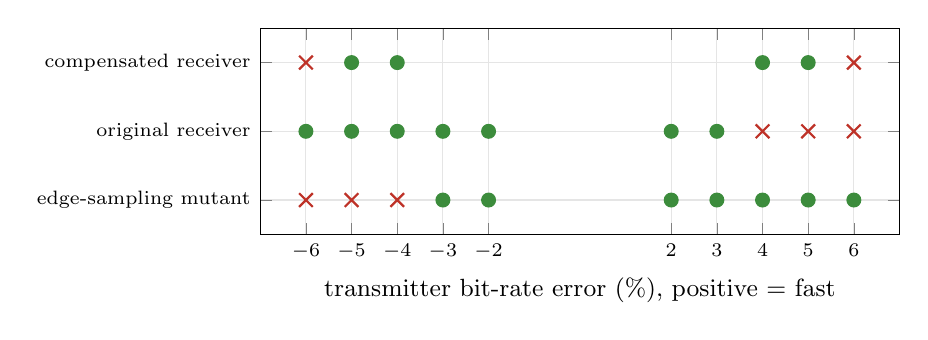
\begin{tikzpicture}
\begin{axis}[width=0.8\linewidth,height=42mm,xmin=-7,xmax=7,ymin=-0.5,ymax=2.5,
  ytick={0,1,2},yticklabels={edge-sampling mutant,original receiver,compensated receiver},
  yticklabel style={font=\scriptsize},xlabel={transmitter bit-rate error (\%), positive = fast},
  xlabel style={font=\small},xtick={-6,-5,-4,-3,-2,2,3,4,5,6},ticklabel style={font=\scriptsize},
  grid=major,grid style={gray!20}]
  \addplot[only marks,mark=*,okc,mark size=2.5pt] coordinates {
    (-6,1)(-5,1)(-4,1)(-3,1)(-2,1)(2,1)(3,1)
    (-5,2)(-4,2)(4,2)(5,2)
    (-3,0)(-2,0)(2,0)(3,0)(4,0)(5,0)(6,0)};
  \addplot[only marks,mark=x,badc,mark size=3.5pt,thick] coordinates {
    (4,1)(5,1)(6,1)
    (-6,2)(6,2)
    (-6,0)(-5,0)(-4,0)};
\end{axis}
\end{tikzpicture}
\caption{UART receiver decoding at 16 clocks per bit, with dots for pass and crosses for fail. The original receiver failed a fast transmitter, and latency compensation centres the window at $\pm5\%$.}
\label{fig:tol}
\end{figure}

\subsection{Receiver bit-rate tolerance}\label{sec:tol}
Every receiver here starts its bit timer from one synchronisation at the start of a frame, so phase error accumulates.
Sweeping the transmitter bit rate in the testbench gives the tolerances in Table~\ref{tab:tol}.

\begin{table}[h]
\centering\small
\caption{Measured tolerance to transmitter bit-rate error, before and after the two fixes.}\label{tab:tol}
\begin{tabularx}{\linewidth}{@{}lccL@{}}
\toprule
Receiver & Before & After & Specification expects \\
\midrule
UART, 10-bit frame & $+6/-4\%$ & $\pm5\%$ & about $\pm5\%$ \\
CAN receive, 500\,kb/s & $+0.35/-0.45\%$ & $\pm0.7\%$ on the test frames & resynchronisation on each edge \\
USB low speed, 1.5\,Mb/s & $+0.4/-0.6\%$ & unchanged & $\pm1.5\%$ \\
MIL-STD-1553, 20-bit word & $-0.2/+0.5\%$ & $-0.25/+0.7\%$ & bit rate $\pm0.1\%$, so covered \\
\bottomrule
\end{tabularx}
\end{table}

Two fixes were applied.
Each receiver subtracts the 3-cycle edge-detection latency from its first half-bit delay, which centres the window.
The CAN and USB data loops also hard-sync on stuff bits: when the stuffing unit reports a stuff bit is due, the next bit is the complement of the current line level, so the firmware waits for that edge and re-anchors the timer.

The second fix is data dependent, and that is its limitation.
Stuff bits follow a run of equal bits, so a frame without long runs produces no resync events and the tolerance stays at the free-running value.
CAN improved on the test frames because they carry 0xFF data, while the USB test packets hold no run of six ones and did not improve at all.
Bit stuffing guarantees a transition at least every 5 bits in CAN and every 7 in USB~\cite{can,usb}, but not at a time the firmware can predict, and only a predictable edge can be waited for.

The general fix is a hardware hard-sync: a configuration bit naming a pin whose edges clear the \sig{since} counter, so the deadline timer re-anchors on every line transition.
That is what CAN resynchronisation and a USB clock-recovery loop do.
The cost is about ten flip-flops in the engine plus matching changes to the Python and Lean models, the differential test, and the mutants.
It is not implemented.
The default test runs include CAN frames at $\pm0.3\%$ and a USB packet at $-0.3\%$, so a loss of margin fails the suite.

\subsection{Protocol tests}
The expanded cocotb suite contains 36 top-level tests, covering protocol behavior and shared resources through the SPI host port. The original 25-test regression passed with behavioral memory, the IHP SRAM functional model and the two-engine flip-flop store. The 36-test suite passed with the four-engine SRAM RTL build, and all 36 tests passed again in gate-level simulation after ASIC hardening.
The directed test \fw{four_engines} runs UART TX, CAN TX, UART RX, and a second UART TX on four engines at once and resets one engine during traffic.
Timing checks against protocol limits cover I2C SCL, MDIO MDC, 1-Wire pulses, WS2812, DMX512, LIN, UART, Modbus silence, the 1553 edge grid, and Ethernet link pulses.
These checks found two firmware defects, an I2C SCL low time of 1.0\,$\mu$s and a 1-Wire reset of 479.9\,$\mu$s.

\subsection{Incidents in the verification process}
An interrupted RTL mutation run once left a mutant in \texttt{src/pe\_core.v}.
The baseline check of the next run caught it.
The file was restored from the previously delivered archive and compared by diff, and the one synthesis run that used the mutant was repeated.
Both mutation scripts now work on private copies, and each regression checks the source tree against an MD5 list.
Review of suspicious results also found several test-harness errors.
They include a miscounted word total, fixed waits that became too short at a new clock, and an invalid initial bus state.

%======================================================================
\section{ASIC physical implementation and timing}

\subsection{Synthesis and floorplan}
The default ASIC uses four IHP 256$\times$16 SRAM macros in an SG13CMOS5L 8$\times$4 tile allocation. A preliminary Yosys 0.69 synthesis with black-box SRAM estimated 0.142\,mm$^2$ in standard cells and 0.112\,mm$^2$ in macros. The physical-design flow subsequently placed and routed the four-engine design, added clock and timing-repair cells, and generated the final GDS.

Four SRAM macros are positioned explicitly in \texttt{src/config.json}; macro supplies are tied into the configured power network through the project's PDN extension. The 20\,ns clock constraint (50\,MHz) is stricter than the design's nominal 48\,MHz operating target.

\begin{table}[!htbp]
\centering\small
\caption{Final placed-and-routed area and instance statistics.}\label{tab:area}
\begin{tabularx}{\linewidth}{@{}lL@{}}
\toprule
Die outline & $1724.16\times710.64\,\mu$m \\
Die area & 1.2253\,mm$^2$ \\
Core area & 1.2082\,mm$^2$ \\
Standard-cell area & 0.2212\,mm$^2$ \\
SRAM macro area (four) & 0.1125\,mm$^2$ \\
Combined cell and macro area & 0.3337\,mm$^2$ \\
Reported core utilization & 27.62\% \\
Standard-cell instances & 14,955 \\
Sequential-cell instances & 1,335 \\
SRAM instances & 4 \\
\bottomrule
\end{tabularx}
\end{table}

The difference from the pre-layout synthesis estimate includes clock-tree cells, hold and setup repair, and other physical implementation changes. SRAM provides about one-third of the combined cell and macro area and stores all four independently programmable instruction memories.

\subsection{Post-route static timing}
Multi-corner post-route static timing analysis checks the 20\,ns target at the fast, typical and slow SG13CMOS5L corners. Table~\ref{tab:corners} reports the worst slack for each corner. Total negative slack and the number of setup and hold violations are zero at all three.

\begin{table}[!htbp]
\centering\small
\caption{Final post-route setup and hold timing (20\,ns clock constraint).}\label{tab:corners}
\begin{tabular}{@{}lcccc@{}}
\toprule
Corner & Voltage & Temp. & Setup slack & Hold slack \\
\midrule
Fast & 1.32\,V & $-40^\circ$C & $+12.6413$\,ns & $+0.1025$\,ns \\
Typical & 1.20\,V & $25^\circ$C & $+10.9540$\,ns & $+0.2800$\,ns \\
Slow & 1.08\,V & $125^\circ$C & $+6.3437$\,ns & $+0.5968$\,ns \\
\bottomrule
\end{tabular}
\end{table}

The original ideal-clock, pre-layout analysis found a hold-sensitive path from the SRAM fetch loop into macro address pins. The final routed design has positive hold slack after clock-tree synthesis and timing repair. With 6.344\,ns worst setup margin under the 50\,MHz constraint, the nominal 48\,MHz operating frequency is supported by the completed static timing analysis.

\subsection{Physical checks and gate-level regression}
\begin{table}[!htbp]
\centering\small
\caption{ASIC implementation and verification results.}\label{tab:asicchecks}
\begin{tabularx}{\linewidth}{@{}lL@{}}
\toprule
GDS hardening & Completed \\
Detailed-route DRC & 0 errors \\
Layout-versus-schematic (LVS) & 0 mismatches \\
Tiny Tapeout precheck & All reported checks passed \\
Post-layout gate-level cocotb & 36 passed, 0 failed \\
Layout render & Generated \\
\bottomrule
\end{tabularx}
\end{table}

The final reports also record 37 maximum-slew and 11 maximum-capacitance violations and 17,712 power-grid violations from an intermediate checker configured not to fail the run on those findings. These results are preserved in the flow logs, alongside the passing DRC, LVS and gate-level regression. The generated GDS, extracted views, and physical reports are available as artifacts of the repository's \texttt{gds.yaml} workflow.

%======================================================================
\section{FPGA implementation and hardware testing}

The same four-engine architecture was implemented on a Digilent Basys3 using inferred block RAM instruction memories and a 48\,MHz clock. An Analog Discovery~3 (AD3) supplied host SPI commands and digital stimulus and captured the resulting waveforms using Digilent WaveForms. Firmware was loaded over SPI rather than compiled into the FPGA bitstream, validating runtime program replacement and the host-controlled configuration path.

\subsection{Vivado implementation}
\begin{table}[!htbp]
\centering\small
\caption{Basys3 resource utilization and post-implementation timing.}\label{tab:fpga}
\begin{tabularx}{\linewidth}{@{}lL@{}}
\toprule
LUTs & 2,597 / 20,800 (12.49\%) \\
Slice registers & 1,362 / 41,600 (3.27\%) \\
RAMB18E1 & 4 / 100 (4.00\%) \\
DSPs & 0 \\
Worst setup slack & $+7.342$\,ns \\
Worst hold slack & $+0.063$\,ns \\
Setup/hold total negative slack & 0\,ns \\
System clock & 48\,MHz \\
\bottomrule
\end{tabularx}
\end{table}

Vivado's timing report states that all user-specified timing constraints are met. Full post-implementation reports are in \path{fpga/results/timing_impl.rpt} and \path{fpga/results/utilization_impl.rpt}.

\subsection{Four-engine concurrency}
Four independently programmed engines produced simultaneous square waves at approximately 6, 12, 24, and 48\,kHz on assigned pins. Measured frequencies were 6.0002, 11.999, 24.001 and 48.000\,kHz, with nearly 50\% duty cycles. This tests concurrent instruction execution, independent timers and memories, and the exclusive pin-routing configuration.
\pescreenshot{four_engines}{Four independent engines running simultaneously, with WaveForms measurements for all four signals.}{fig:fpga-four}

\FloatBarrier
\subsection{UART and SPI}
At 38,400 baud, UART TX generated repeated \texttt{0x55} data with a measured 26.071\,$\mu$s bit period. An externally driven UART RX test returned \texttt{0x55}, \texttt{0xAA}, \texttt{0x00}, and \texttt{0xFF} in the expected FIFO order. The SPI test generated mode-0 transactions near 100\,kHz, transmitting \texttt{0x69}; an external \texttt{0x96} transfer was received as \texttt{0x0096} through the host readback path.
\pescreenshot{uart_tx}{UART TX at 38,400 baud, decoded as repeated \texttt{0x55} bytes.}{fig:fpga-uart}
\pescreenshot{spi_tx}{Mode-0 SPI transmission near 100\,kHz, with \texttt{0x69} decoded on MOSI.}{fig:fpga-spi}

\FloatBarrier
\subsection{I\textsuperscript{2}C and 1-Wire}
I\textsuperscript{2}C controller firmware generated START, address \texttt{0x50}, acknowledgment phase, and STOP on open-drain SCL and SDA. A second engine acted as an ACK responder; the master observed SDA LOW on the ninth SCL pulse and returned the expected result through its RX FIFO.
\pescreenshot{i2c_tx}{I\textsuperscript{2}C master address and data timing captured on SCL and SDA.}{fig:fpga-i2c}

The 1-Wire waveform included a reset interval of approximately 481\,$\mu$s, a 6.3\,$\mu$s write-one LOW pulse, a 60\,$\mu$s write-zero LOW pulse and 70\,$\mu$s slots. A second engine provided a slave presence response. The master distinguished the responding and nonresponding cases, returning \texttt{0x0000} and \texttt{0x0001}, respectively.
\pescreenshot{onewire_tx}{1-Wire reset and write-slot timing, with cursor measurements.}{fig:fpga-onewire}

\FloatBarrier
\subsection{Manchester, NRZI, and PWM}
Manchester TX measured a 9.885\,$\mu$s bit period and 4.970\,$\mu$s half-bit interval. Inter-engine RX loopback recovered test frames including \texttt{0x96}. For continuous streaming, backpressure could interrupt the simplified receiver and cause later loss of alignment; individual frame encoding and decoding were confirmed.
\pescreenshot{manchester_tx}{Manchester-coded output with measured bit and half-bit intervals.}{fig:fpga-manchester}

The NRZI loopback used the engine's built-in encoder and decoder. One engine transmitted \texttt{0xA6}; another returned \texttt{0xA600} through the RX FIFO. This exercises physical pin sampling and serial line decoding.

Two PWM programs used ordinary deadline and pin-control instructions to generate a nominal 12\,kHz waveform with 25\% and 75\% duty settings. Table~\ref{tab:pwm} summarizes the measured frequencies and pulse widths.

\begin{table}[!htbp]
\centering\small
\caption{Measured FPGA PWM signals.}\label{tab:pwm}
\begin{tabular}{@{}lcc@{}}
\toprule
Measurement & 25\% setting & 75\% setting \\
\midrule
Frequency & 11.999\,kHz & 12.000\,kHz \\
Period & 83.340\,$\mu$s & 83.330\,$\mu$s \\
Duty cycle & 24.982\% & 74.979\% \\
HIGH interval & 20.820\,$\mu$s & 62.480\,$\mu$s \\
LOW interval & 62.520\,$\mu$s & 20.850\,$\mu$s \\
\bottomrule
\end{tabular}
\end{table}
\begin{figure}[!htbp]
\centering
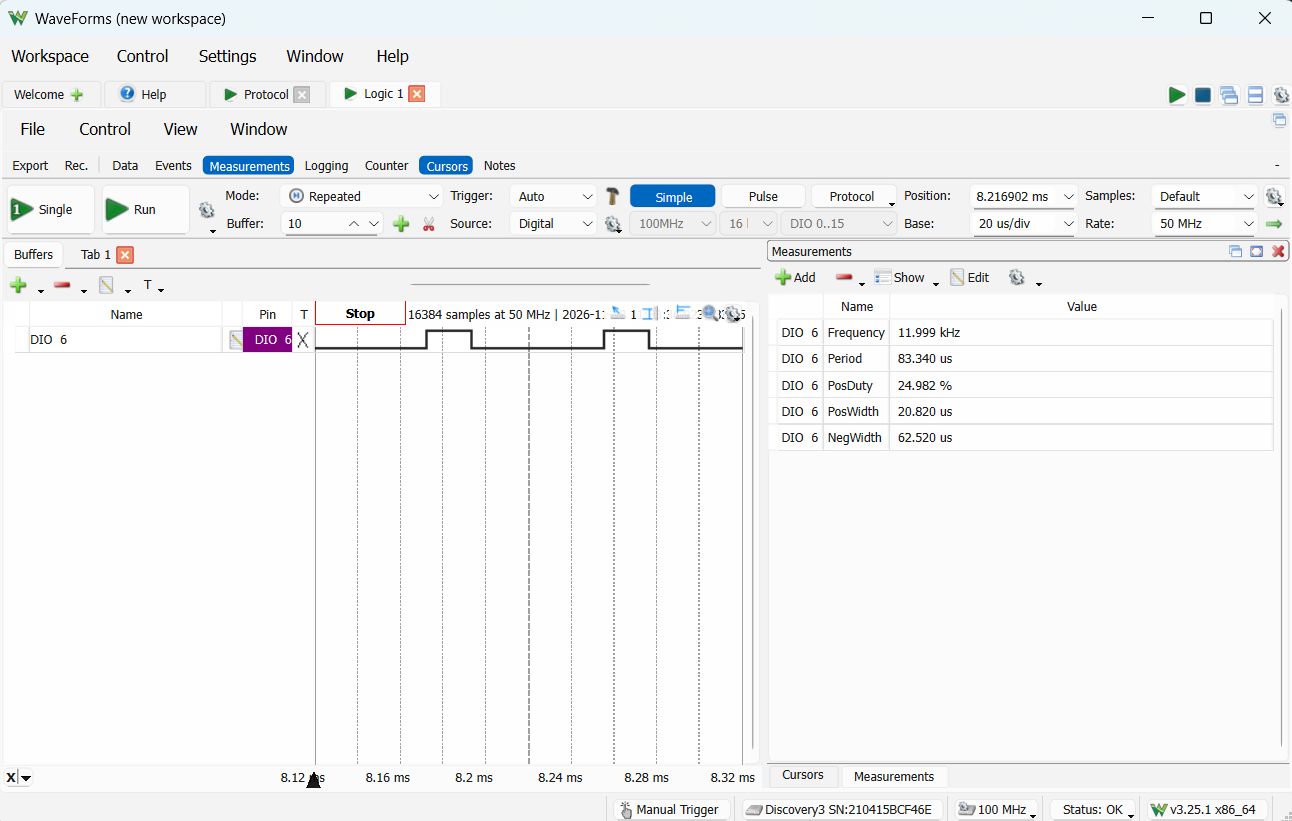
\includegraphics[width=0.49\linewidth,keepaspectratio]{../../fpga/results/screenshots/pwm_25.png}\hfill
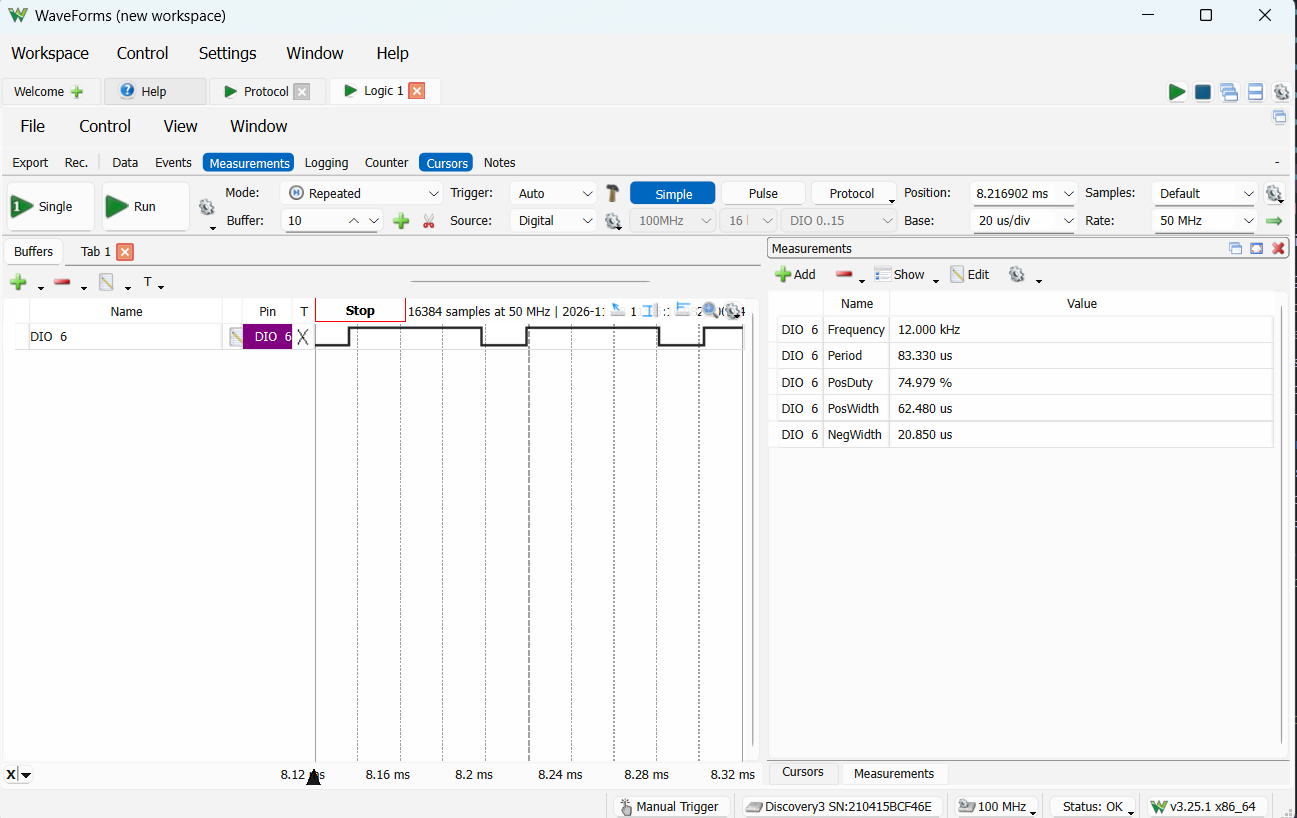
\includegraphics[width=0.49\linewidth,keepaspectratio]{../../fpga/results/screenshots/pwm_75.png}
\caption{FPGA PWM captures: 24.982\% duty cycle (left) and 74.979\% (right), both near 12\,kHz.}
\label{fig:fpga-pwm}
\end{figure}

Hardware tests also exercised SPI firmware loading, stop/restart, per-engine reset, TX/RX FIFO transfers, owner/validity-mask configuration and configuration readback. Test scripts and all eight captures are under \texttt{fpga/tests/} and \texttt{fpga/results/screenshots/}, respectively.
\FloatBarrier

%======================================================================
\section{Design trade-offs and future work}\label{sec:issues}

The instruction set emphasizes shared signaling mechanisms rather than specialized peripheral controllers. This enables many interfaces with the same four cores, while the maximum rate of a program depends on the instruction count along each bit's critical firmware path. The Manchester Ethernet program, for example, demonstrates framing and link pulses at 2\,Mb/s rather than full 10BASE-T speed.

The synchronization strategy is similarly programmable. Receivers compensate the input synchronizers' detection latency and, where useful, re-anchor timing on known line transitions. Hardware-assisted edge synchronization could extend CAN and USB clock tolerance with less firmware overhead. Higher-level protocol features such as USB enumeration, full CAN arbitration/error recovery, and MIL-STD-1553 terminal scheduling can be implemented in host software or added to firmware over time.

The final output-ownership mux removes the earlier cross-engine pin-combining problem. The shared input network still lets any engine observe a line, while pin assignments can be changed without resynthesizing the design. More protocol pins or deeper buffering would require additional RTL resources, rather than changes to the core instruction model.

%======================================================================
\section{Reproducing the results}

The following commands are run from the repository root unless noted otherwise.
\begin{lstlisting}[language={}]
make -C test                                   # expanded cocotb suite
make -C test SRAM_MODEL=yes PDK_ROOT=<ihp-pdk> # IHP SRAM model
make -C test IMEM=flop                         # 2-engine fallback
make -C test/core                              # RTL/Python differential
# Mutation campaigns:
test/core/mutate.sh
test/fw_mutate.sh [test-name-prefix]
cd lean && lake build                          # Lean model and proofs
python3 gen_traces.py 500 600 | .lake/build/bin/crosscheck
./run_regression.sh                            # historical complete regression
\end{lstlisting}

The ASIC build, Tiny Tapeout precheck, gate-level simulation and layout render run through the GitHub Actions workflow \texttt{.github/workflows/gds.yaml}. Their outputs are retained as workflow artifacts. FPGA build inputs and host test scripts are in \texttt{fpga/basys3/} and \texttt{fpga/tests/}, while the reports and screenshots are in \texttt{fpga/results/}. Full methodology and measurement context are provided in \texttt{docs/verification.md}.

%======================================================================
\section*{References}
\addcontentsline{toc}{section}{References}
\small
The reference models in the testbench follow the documents below.
Entries marked $\dagger$ were checked against the publisher's document during this work, including revision and date.
For the others the entry gives the defining document for the protocol as implemented, without a verified revision.
CRC check values come from the catalogue of parametrised CRC algorithms \cite{reveng}.

\normalfill
\begin{thebibliography}{99}
\bibitem{js} B. Devlin and A. Singhani, ``Can you design a chip? Announcing the protocol emulator ASIC competition,'' Jane Street Blog, 10 September 2026.$\dagger$
\bibitem{tt} Tiny Tapeout, documentation and CMOS5L Verilog template, \url{https://tinytapeout.com}.$\dagger$
\bibitem{ihp} IHP Microelectronics, IHP-Open-PDK, SG13CMOS5L process design kit, \texttt{dev} branch.$\dagger$
\bibitem{rs232} TIA/EIA-232-F, \emph{Interface Between Data Terminal Equipment and Data Circuit-Terminating Equipment Employing Serial Binary Data Interchange}, Telecommunications Industry Association. Asynchronous 8N1 character framing.
\bibitem{spi} Motorola, \emph{SPI Block Guide}, V03.06, document S12SPIV3/D. Defines clock polarity and phase modes 0 to 3.
\bibitem{i2c} NXP Semiconductors, \emph{I\textsuperscript{2}C-bus specification and user manual}, UM10204, Rev.~7.0, 1 October 2021.$\dagger$ Fast-mode timing in Table~10.
\bibitem{jtag} IEEE Std 1149.1-2013, \emph{IEEE Standard for Test Access Port and Boundary-Scan Architecture}. TAP controller state diagram and IDCODE.
\bibitem{swd} Arm Ltd., \emph{Arm Debug Interface Architecture Specification, ADIv5.0 to ADIv5.2}, IHI0031. Serial wire protocol, request format, turnaround, and DPIDR.
\bibitem{mdio} IEEE Std 802.3, \emph{IEEE Standard for Ethernet}, Clause 22 (MII management interface, MDC and MDIO timing) and Clause 14 (10BASE-T Manchester signalling and link pulses).
\bibitem{ps2} A. Chapweske, ``The PS/2 Mouse/Keyboard Protocol,'' 2003, and IBM, \emph{Personal System/2 Hardware Interface Technical Reference}, 1990.
\bibitem{onewire} Maxim Integrated (now Analog Devices), Application Note 126, \emph{1-Wire Communication Through Software}, and the DS18B20 data sheet. Standard-speed reset, presence, and slot timing.
\bibitem{ws2812} Worldsemi, \emph{WS2812B Intelligent Control LED Integrated Light Source}, data sheet. Bit period 1.25\,$\mu$s with 0.4 and 0.8\,$\mu$s high times.
\bibitem{dmx} ANSI E1.11, \emph{USITT DMX512-A, Asynchronous Serial Digital Data Transmission Standard for Controlling Lighting Equipment and Accessories}, Entertainment Services and Technology Association. Break, mark after break, and 250\,kbaud 8N2 slots.
\bibitem{lin} ISO 17987 series, \emph{Road vehicles: Local Interconnect Network (LIN)}, and LIN Consortium, \emph{LIN Specification Package}, Revision 2.2A, 2010. Break field, sync byte, protected identifier, and checksum.
\bibitem{can} ISO 11898-1, \emph{Road vehicles: Controller area network (CAN), Part 1: Data link layer and physical signalling}, and Robert Bosch GmbH, \emph{CAN Specification}, Version 2.0, 1991. Frame format, bit stuffing, and the CRC-15 polynomial 0x4599.
\bibitem{usb} USB Implementers Forum, \emph{Universal Serial Bus Specification}, Revision 2.0, 27 April 2000. Low-speed signalling, NRZI, bit stuffing, packet formats, CRC-5 and CRC-16.
\bibitem{modbus1} Modbus Organization, \emph{MODBUS over Serial Line Specification and Implementation Guide}, V1.02, 20 December 2006.$\dagger$ RTU framing, 8E1 characters, and the 3.5-character silence.
\bibitem{modbus2} Modbus Organization, \emph{MODBUS Application Protocol Specification}, V1.1b, 28 December 2006.$\dagger$ Function codes, including read holding registers.
\bibitem{mil1553} MIL-STD-1553B, \emph{Department of Defense Interface Standard, Digital Time Division Command/Response Multiplex Data Bus}, United States Department of Defense, with Notice 2, 1986. Sync patterns, Manchester II coding, and odd parity.
\bibitem{reveng} G. Cook, \emph{Catalogue of Parametrised CRC Algorithms}, \url{https://reveng.sourceforge.io/crc-catalogue/}. Check values for CRC-15/CAN, CRC-16/USB, CRC-5/USB, and CRC-16/MODBUS.
\end{thebibliography}

\end{document}
